  % Template for ICASSP-2019 paper; to be used with:
%          spconf.sty  - ICASSP/ICIP LaTeX style file, and
%          IEEEbib.bst - IEEE bibliography style file.
% --------------------------------------------------------------------------
\documentclass{article}
\usepackage{styles/spconf,amsmath,graphicx,subfig}
\usepackage{multirow}

% MY OWN
\graphicspath{{figures/}}
\newcommand{\x}{\mathbf{x}}
\newcommand{\myr}{\mathbf{r}}
\newcommand{\myw}{\mathbf{w}}
\newcommand{\mya}{\mathbf{a}}
\newcommand{\bea}{\mathbf{b}}
\newcommand{\z}{\mathbf{z}}
\newcommand{\Hist}{\mathbf{H}}
\usepackage[hidelinks]{hyperref}
\usepackage{mathtools,bbm}
\usepackage{tikz}
\usetikzlibrary{bayesnet}

% Example definitions.
% --------------------
%\def\x{{\mathbf x}}
%\def\L{{\cal L}}

% Title.
% ------
\title{RADIO MAP ESTIMATION WITH NEURAL NETWORKS AND ACTIVE LEARNING FOR INDOOR LOCALIZATION}
%
% Single address.
% ---------------

\name{S\i{}la G\"{u}ler$^{\star}$ \qquad F. Serhan Dani\c{s}$^{\star\dagger}$ \qquad Ali Taylan Cemgil$^{\star}$}

\address{$^{\star}$ Department of Computer Engineering, Bo\u{g}azi\c{c}i University, Istanbul 34342, Turkey \\
		$^{\dagger}$Department of Computer Engineering, Galatasaray University, Istanbul 34349, Turkey}
%
% For example:
% ------------
%\address{School\\
%	Department\\
%	Address}
%
% Two addresses (uncomment and modify for two-address case).
% ----------------------------------------------------------
%\twoauthors
%  {A. Author-one, B. Author-two\sthanks{Thanks to XYZ agency for funding.}}
%	{School A-B\\
%	Department A-B\\
%	Address A-B}
%  {C. Author-three, D. Author-four\sthanks{The fourth author performed the work
%	while at ...}}
%	{School C-D\\
%	Department C-D\\
%	Address C-D}
%
\begin{document}
	%\ninept
	%
	\maketitle
	%
	\begin{abstract}
		Practical indoor localization, by exploiting electromagnetic scattering properties of local area networks, can be formulated as a tracking problem using a Hidden Markov model (HMM). In order to use as the observation model of the HMM, neural networks are used for generating a radio frequency map over an indoor location. Accurate estimation of the radio map is key in accurate localization but this requires dense sampling of the electromagnetic field, also named as fingerprinting. To decrease the time consuming fingerprinting process, we follow an active learning strategy based on uncertainty sampling aided by a Gaussian process. Our results indicate that the same localization performance can be maintained with less fingerprint measurements using our approach.
	\end{abstract}
	%
	\begin{keywords}
		Indoor localization, neural networks, radio map estimation, uncertainty sampling
	\end{keywords}
	%
	\section{INTRODUCTION}
	\label{sec:intro}
	Localization, stated also as positioning or geolocation, has become a widespread research area since 2000s. This substantial increase is originated from the extensive use cases of position estimation in marketing, healthcare \cite{Cal2015}, asset tracking and robotics in emergency scenarios like fire and mine accidents \cite{Zha2009}. With the help of GPS technology, studies have achieved approximately 10 meters localization accuracy outdoor \cite{Dju2001}. However, GPS signals cannot be used for indoor localization because they are faded in indoor spaces due to the destructive multi-path signal propagation and dense obstacles shadowing the signal \cite{bah2000,Bat2002}. Although various other techniques have been studied for indoor localization, there is still room for progress to decrease the localization error. 
	
	Indoor localization approaches are mainly divided into three sub categories: geometry-based, propagation-based and fingerprinting-based techniques. In geometry based approaches the position of the object is found by using Time of Arrival (TOA), Time Difference of Arrival (TDOA) or Angle of Arrival (AOA) information with triangulation principle \cite{Fan1990,Pet1998}, but its main drawback is that these techniques cannot model the multi-path and shadowing effect. In propagation based approaches \cite{bah2000}, attenuation of signal power is modeled with various radio propagation models. The power of radio signals can be based on various parameters like transmitter distance and wall attenuation factor. Though radio propagation based models are successful to model multi-path and shadowing effects, this procedure should be repeated because of the attenuation characteristic of each environment. The most reliable technique, fingerprinting is composed of two phases. The first phase is collecting reduced signal strength indicator (RSSI) values at specified locations in a place and constructing a radio frequency map (RM) from this collected information. The second phase is location estimation based on this RM with several estimation methods such as k-Nearest Neighbor ($k$NN), Neural Networks (NN), Support Vector Machines (SVM) and Kernel Density Estimators \cite{Roo2002}. In $k$NN approach \cite{bah2000,Big2017}, when a new RSSI is observed from an unknown location, $k$ location candidates having the closest RSSI value are selected. Weighted or unweighted average of these candidate locations gives the location estimate. On the other hand, NNs are used for generating radio maps, where the relationship between RSSI information and locations are too complex to be solved with other techniques \cite{Lyu2011,Maz2015,Sol2016,Zho2017}. An estimate for the most probable position is finally inferred by choosing the position that maximizes the probability given the signal strength measurement \cite{Fas2016}, therefore, they are effective for discrete positioning. 
	
	% Considering these researches, we concluded the following. Modeling the RSSI values at each location with a propagation model has to be site specific, because in each side attenuation factors change. Therefore, it's very time consuming. Generating a deterministic radio map, by taking the mean or median over RSSI samples, causes losing the information of how signal strengths change with time and less accurate positioning than one with probabilistic radio map generation. Localization with probabilistic models like kernel method is a good choice because it gives approximately 1.5 meter accuracy on average \cite{Roo2002}. However, in order to follow this approach, we need to find the kernel function class which is the most appropriate for our observations. With the non-linear transformations in each neuron at each layer, Neural networks are successful in modeling the complex relationship between RSSI strengths and locations. In the great majority of researches, they are used directly for estimating the location given RSSI information. Most studies base location prediction model on the collected fingerprints. However, fingerprint collection is time consuming. Therefore, estimating the fingerprints in a dense grid of locations, and making predictions based on the radio map with estimated fingerprints is a better method saving measurement cost. BLE beacons require low energy for transmitting RF signals. Therefore, their battery life is longer than the one of Wi-Fi transmitters. As \cite{Maz2015} stated BLE beacons enable signals to transmit further distances so they are more appropriate for localization purposes. 
	% 	Modeling the RSSI values at each location with a propagation model has to be site specific because attenuation factors change. 
	% 	
	Generating a deterministic radio map, by taking the mean or median over RSSI samples, causes losing the information of how signal strengths change with time. Localization with kernel methods achieve great accuracy \cite{Roo2002} but determining an appropriate function class is very hard. NNs are mostly used directly for estimating the location given RSSI information. Moreover, prediction models are mostly based on the collected fingerprints. To reduce the time spent on fingerprint collection, it's better to estimate in a dense grid of locations from the collected fingerprints. With the motivation of accurate indoor localization without collecting too many fingerprints, we propose the method of Radio Map Estimation with Neural Networks and Active Learning. We consider tracking problem as a time series problem and model it with Hidden Markov model (HMM) which provides us an estimation affected by the previous locations. To use in the observation model, we generate a probabilistic radio map by estimating the signal distribution at any position based on the collected fingerprints. To do so, we use neural networks. Novelty in this study is that we reduce the number of fingerprints to be used as training fingerprints for the neural networks by using a Gaussian Process (GP). %and uncertainty sampling approach.
	
	%Finally, BLE beacons require low energy for transmitting RF signals. 
	
	The rest of the paper is organized as follows: In Section~\ref{sec:methodology}, we explain the proposed methods. In Section~\ref{sec:experiments} we give the details of experiments and discuss the achieved results and we conclude with Section~\ref{sec:conclusion}.
	
	\section{METHODOLOGY}
	\label{sec:methodology}
	We consider the tracking problem inference in HMM \cite{barberBRML2012} in which observations are the RSSI measurements and the latent variables are the positions of the receiver. With an observation at hand at a time, together with the previous observations, we aim inferring the current position. For the transition model, a diffusion motion model is selected as explained in \cite{Ser2017}. On the other hand, for the observation model, we provide a probabilistic radio map as a lookup matrix storing the probability distributions of RSSI values at a given position. Having transition and observation model at hand, we use Sequential Monte Carlo (SMC) to compute the filtering distribution and select the most likely position of this distribution as the candidate location.
	
	To generate a probabilistic radio map in a dense grid of locations, we use NNs which are successful to model complex relationships as in between RSSI distribution measured at a position and the position itself. 
	
	In order to select training fingerprints for the neural networks, we employ an active learning strategy. %To determine a valid configuration of a predetermined number of fingerprints, we employ an active learning strategy. 
	This strategy automates the fingerprint selection procedure with uncertainty sampling, which suggests selecting the fingerprints with lowest confidence values. We make use of the Gaussian Processes (GP) to model the uncertainty at map positions.
	
	\subsection{Radio Map Estimation}
	We train a Single Layer Neural Network (SNN) with five different feature sets and different hidden unit sizes. Based on the concern that an SNN is not successful enough to generalize the function between our input features and output, we train a Deep Neural Network (DNN) with two hidden layers.
		
	As input features, five different sets, $\mathcal{S}_i$, are constructed with different combinations of the distances between the beacon and the receiver, RSSI histograms (fingerprints) on the neighboring positions and their distances to the transmitter (see \tablename{~\ref{tab:features}} for details). In the input layer, we feed the features and in the output layer we have the discrete probability distributions (histograms) of RSSI values with indexes ranging from $-100$ to $-20$. 
	%At each layer, activation units are computed as in (\ref{eq:activation}). 
	As the loss function, we select Squared Earth Mover's Distance (EMD$^2$)\cite{Rub2000} which corresponds to the sum of squares of element-wise difference between the cumulative distribution functions (CDF) of original and predicted distributions. In an ordered multi-class classification problem they become equivalent to Mallow's distance, without the normalization term, its closed form solution is stated as \cite{conf/iccv/LevinaB01}, \cite{Hou2016}:
	\begin{small}
		\begin{align}
		\begin{split}
		\text{EMD}^2(p, q) &\propto || F_P(p) - F_Q(q)||^2_2 \end{split}
		\end{align}
	\end{small}
	where $p$ and $q$ are original and predicted distributions to be compared, $F_P(p)$ and $F_Q(q)$ are the cumulative distribution functions. For hidden and output layers, we select a sigmoid as one of the most commonly used activation function. Comparing the results of feature sets and unit size on the validation data, we choose the best setting that minimizes the generalization loss. Both models are trained with the weights and biases initialized with Glorot Initializer \cite{Glo2010} and as zero respectively. Optimum weight and bias values are computed with the back-propagation algorithm. For the optimization, we employ RMSProp optimization algorithm. \cite{Good2016}
	\begin{small}
		\begin{align}
		\begin{split}
		f(\x; W, b, g) = g_3(W_3 g_2(W_2 g_1(W_1 \x + b_1) + b_2) + b_3)
		\end{split}
		\label{eq:model}
		\end{align}
	\end{small}
	where $\x$ is the input vector, $W$'s are weight parameters, $b$'s are bias parameters, $g_1$ is the activation function in the hidden layer, and $g_2$ is the activation function in the output layer.
	%	\begin{small}
	%	\begin{align}
	%		\begin{split}
	%		\mya^{(l)} &= g(\z^{(l)})  \\
	%		\z^{(l)} &= \myw^{(l)} \mya^{(l-1)} + \bea^{(l)}
	%		\end{split}
	%	\label{eq:activation}
	%	\end{align} 
	%	\end{small} where $l$ is the index of the layer, $g$ is the activation function, $\myw^{(l)}$ and $\bea^{(l)}$ are the weight and bias vectors and finally $\mya^{(l)}$ is the activation unit vector in $l^{th}$ layer. 
	\begin{table}[h]
		%\begin{table}[h]
		\centering
		\resizebox{0.75\columnwidth}{!}{
			\begin{tabular}{|c|c|c|}
				\hline
				\textbf{Feature Sets} & \textbf{Features} \\ \hline
				$\mathcal{S}_1$ & $PT$ \\
				\hline
				$\mathcal{S}_2$ & $PF_1, TF_1, \Hist_1$ \\
				\hline
				$\mathcal{S}_3$ & $PF_{1,2} TF_{1,2}, \Hist_{1,2}$ \\
				\hline
				$\mathcal{S}_4$ & $PF_{1,2,3}, TF_{1,2,3}, \Hist_{1,2,3}$ \\
				\hline
				$\mathcal{S}_5$ & $PT, PF_{1,2,3,4}, TF_{1,2,3,4}, \Hist_{1,2,3,4}$ \\
				\hline
			\end{tabular}
		}
		
		\caption{Input Features: $PT$ stands for the distance of the position to the transmitter, $PF_i$ for the distance of the position to the $i^{th}$ closest fingerprint, $TF_i$ for the distance between the $i^{th}$ closest fingerprint and the transmitter and $\Hist_i$ for the histogram on the $i^{th}$  closest fingerprint, with indexes depicting the rank of the proximity.}		
		\label{tab:features}
	\end{table} 
	\subsection{Active Learning with Gaussian Processes}
	We use a GP to model mapping functions between positions and RSSI values. Using the correlation between positions function value in a new position is calculated. 
	\begin{small}
		\begin{align}
		\begin{split}
		f(\x) &\sim \mathcal{GP}(m(\x), K(\x,\x)) \\
		\text{i.e. \ } f(\x) &\sim \mathcal{N}(m(\x), K(\x,\x))
		\end{split}
		\label{eq:GPRMath}
		\end{align} where
		\begin{align}
		k(\x_i,\x_j) = 
		\left\{
		\begin{array}{ll}
		\sigma_f\exp\Big(-\frac{\displaystyle 1}{\displaystyle 2l^2}\left\Vert(\x_i-\x_j)\right\Vert^2_2 \Big)  & \mbox{if } i \neq j \\
		\sigma_n^2 + \sigma_f\exp\Big(-\frac{\displaystyle 1}{\displaystyle 2l^2}\left\Vert(\x_i-\x_j)\right\Vert^2_2 \Big) & \mbox{if } i = j
		\end{array}
		\right.
		\end{align}
	\end{small}
	where $m(\x)$ is the mean of the Gaussian distribution of the random variable $\x$ and $K(\x,\x)$ is the covariance function. Covariance functions are used to reflect the correlation between inputs to function values. In our case, distance between the locations make difference in RSSI values regardless of its direction. Therefore, squared exponential function is selected as the covariance function of GP. The covariance matrix is parametrized by $k(\x_i,\x_j)$, and $\sigma_{f}$, $l$ and $\sigma_{n}$ are the hyper-parameters of the model. We find the optimum hyper-parameters with gradient ascent by maximizing the log marginal likelihood as in \cite{Ras2006}. A strategy, based on predictive variance, is used as the criteria for fingerprint selection. For each transmitter a random fingerprint is selected as the first training location to train the GP once. At each subsequent step of the selection strategy, the fingerprint which has the greatest variance is chosen to be included in the training set. Retraining with the newly added fingerprint, predictive variance for the remaining locations are calculated and this procedure continues until we reach the target number of fingerprints. An important remark is that to model the mapping function with a GP, a single RSSI value is used as the output. Therefore, we need to take one value out of the signal strength distribution and the best candidate is the most probable value which corresponds to the mode of the distribution. 
	
	\section{EXPERIMENTS And RESULTS}
	\label{sec:experiments}
	We conduct our experiments on two different datasets, collected from two different areas:  
	%\subsubsection{Synthetic Fingerprints}
	%To test the proposed algorithms for radio map generation with Neural Network, we sample synthetic fingerprints that imitate the true histograms formed with the measured RSSI data. We model a very simple toy sampler, in which the histograms are discretized Gaussians, whose means depend on a distance measure between the positions of transmitter(i.e. beacon), $\bea$, and the receiver, $\x$. The mathematical model is given as in (\ref{eq:generativemodel}), and the corresponding graphical model can be seen in \figurefname~\ref{fig:graphicalmodel}.
	%\begin{align}
	%\begin{split}
	%\mu &= g(\left\Vert(\x - \bea)\right\Vert) \\
	%\mathcal{R} &\sim \mathcal{N}(\mu, \sigma^2)
	%\end{split}
	%\label{eq:generativemodel}
	%\end{align}
	%\begin{figure}[h]
	%	\centering
	%	\resizebox{0.5\columnwidth}{!}{
	%	\tikz{
	%		\node[latent](x) {$\x$};
	%		\node[latent][right= of x] (b) {$\bea$};
	%		\node[latent][below=of x] (mu) {$\mu$};
	%		\node[obs][below= of mu](r1) {$r_{1}$};
	%		\node[obs][right= of r1] (r2) {$...$};
	%		\node[obs][right= of r2] (r3) {$r_{i}$};
	%		\node[obs][right= of r3] (r4) {$...$};
	%		\node[obs][right= of r4] (rK) {$r_{K}$};
	%		\node[const][right= of mu] (sigma) {$\sigma$};
	%		\edge {x,b} {mu};	
	%		\edge {mu,sigma} {r1,r2,r3,r4,rK};	
	%		\plate {rr} {(r1)(rK)} {$i: 1..K$};
	%		\plate {yx} {(x)(b)(rr)} {}  } }
	%	\caption{Graphical Model of Generative Model}
	%	\label{fig:graphicalmodel}
	%\end{figure}
	%We aim to generate a mean value, $\mu$, for the Gaussian using a scaling function of the Euclidean Norm of the distance, $g(\left\Vert(\x - \bea)\right\Vert)$. We also set the variance, $\sigma^2$, to a constant real number. With $\mu$ and $\sigma^2$, we have a Gaussian distribution defined. To make the distribution look like the RSSI histograms, we discretize this distribution on the integer values in a predefined interval. We use this discretized Gaussian as the fingerprint of the beacon $b$ on the location, $\x$. $\mathcal{R} = \{r_i\}_{i=1}^{K}$ stands for fingerprint histogram where $r_i$ defines the probability measure of the $i^{th}$ RSSI value and $K$ represents the total number of discrete RSSI values.
	%We assume to have a two dimensional map in $R^2: U \times V$ where $U=\{0,1,...,10\}$ and $V=\{0,1,...,10\}$. From this map, we selected 36 fingerprint locations equidistantly. They are divided into training, validation and test randomly with the percent of 70-15-15. So, we got 25 locations as training, 5 as validation and 6 as test. 
	%\begin{align*}
	%\begin{split}
	%\x &\in S \times W \text{, where } S=\{0, 2, ..., 10\} \text{ and } W=\{0, 2, ..., 10\} \\
	%\bea &\in \{(5,0),(0,5),(5,10),(10,5)\}
	%\end{split}
	%\end{align*}
	%%\textbf{Probability Distribution Generation}:
	%To simulate RSSI value distribution we calculate the mean from \ref{eq:gfunc}. $\alpha$ and $\beta$ are set to the following numbers in order to map the scale of distance to the scale of RSSI values. So that, at the closest location to a beacon, which has $0m$ distance to it, we have the mean RSSI value as $-30$ whereas at the furthest location, $14.14$ meter far from it, we have the mean RSSI value as $-90$. 
	%\begin{align}
	%\begin{split}
	%g(\left\Vert(\x-\bea)\right\Vert) &= \alpha \left\Vert(\x-\bea)\right\Vert +\beta \\
	%\alpha &= -4.25 \\
	%\beta &= -30
	%\end{split}
	%\label{eq:gfunc}
	%\end{align}
	%For RSSI values ranging from $-100$ to $-20$, we calculate the probability from the Gaussian Distribution formula below.
	%\begin{align}
	%\begin{split}
	%p(r) &= \dfrac{1}{Z} \ \phi(r) \\
	%Z &= \sum_{r}\phi(r) \\
	%\phi(r) &= \exp\Bigg(-\dfrac{1}{2} \ \Big(\dfrac{r-\mu}{\sigma}\Big)^{2}\Bigg)
	%\end{split}
	%\end{align}
	The first area, $\mathcal{A}_1$, is a living room ($5.28\times6.35$ m$^2$) containing 6 Bluetooth Low-Energy (BLE) beacons, transmissions of which are logged at 50 locations each for 24 hours \cite{Ser2017} (see \figurename~\ref{fig:Room A_finger}). Discrete RSSI distributions are constructed from the collected data. We use 70\% of the preprocessed data as training, and the remaining for validation and test purposes. The training data are used for calculating the optimum weights and biases, whereas the validation data are left for deciding the best architecture. The test data are used only for evaluating radio map (RM) estimation performance with the specified loss functions. 
	\begin{figure}
		\centering
		\subfloat[$\mathcal{A}_1$]{
			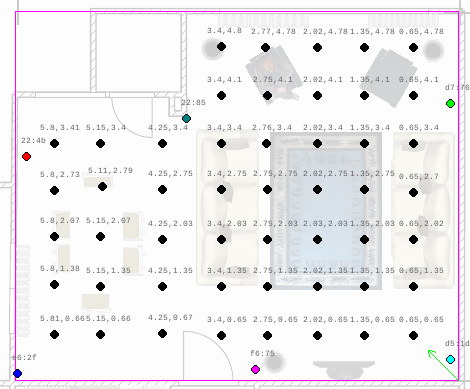
\includegraphics[width=.4\linewidth]{fingerprints_ortakoy.png}
			\label{fig:Room A_finger}}
		\subfloat[$\mathcal{A}_2$]{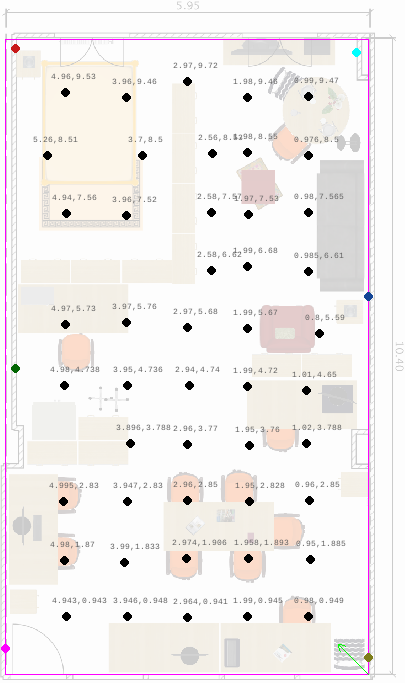
\includegraphics[width=.4\linewidth]{fingerprints_lab8.png}
			\label{fig:Room B_finger}
		}
		
		\caption{Fingerprint distribution of two test areas. Black points represent fingerprint positions and colored ones are the beacons.}
	\end{figure}
	The second area $\mathcal{A}_2$ is a home simulation environment ($10.40\times5.95$ m$^2$) \cite{tunca2014}. Fingerprint data are collected for 20 minutes from 6 beacons mounted on the walls of the area (see \figurename~\ref{fig:Room B_finger}). We follow the same procedure for data manipulation, as we did for the $\mathcal{A}_1$ fingerprints.
	
	All computation is performed on an Intel Core i7 based computer running at 4 GHz and 8GB of RAM. The models are constructed on Keras 2.1.5 \cite{chollet2015} using Tensorflow as its backend. 
	%\subsection{Synthetic Data Experiments}
	%For our synthetic data, we train a single layer neural network for the beacon at the location of (0,5) with different number of hidden units in $(20,520)$. We run RMSProp optimization algorithm for 500 epochs with its default learning rates of 0.001 in order to find the optimum weights. At each epoch, we pass the entire dataset to the network one by one which means our batch size is 1. Optimum hidden unit sizes are observed to be 420 units. Therefore, we use the weights corresponding to 420 units in order to predict RSSI distribution for the test locations. It's seen that they are well suited to the original distributions as in \figurename~\ref{fig:pred_all_generative_MSE}.
	%\begin{figure}[h]
	%	\centering
	%	\includegraphics[width=0.7\columnwidth]{Generative/Pred-Test}
	%	\caption{Predictions on test locations for the beacon at $(0,  5)$ }
	%	\label{fig:pred_all_generative_MSE}
	%\end{figure}
	
	For the test area of $\mathcal{A}_1$, we train a SNN with 5  feature sets as previously stated in Table \ref{tab:features} and 25 different unit sizes for 10 times with each beacon. To train the model 10 times, we construct 10 fingerprint configurations at the beginning by dividing our data into training, validation and test fingerprints randomly and use the same configuration to compare the results of these feature sets. To decide the best architecture, we look at the average validation loss over all beacons. 
	
	\figurename~\ref{fig:RoomA-MSE-All} shows that $\mathcal{S}_1$ yields much greater error than the remaining feature sets, meaning that the estimations depending solely on transmission distances perform very poorly. Although there is not a great difference, among the remaining ones, $\mathcal{S}_4$ gives the minimum EMD$^2$ loss with 60 units in the hidden layer. This can be interpreted as that the best configuration of the feature sets are constructed by the four nearest fingerprint data, transmission distances and their histograms. On the other hand, for training the DNN, we experiment with hidden unit sizes ranging from 10 to 100. While exploring the optimum hidden unit size, we use the same number of units for each layer. We conclude that $\mathcal{S}_4$ and 40 unit is the optimum architecture as seen in \figurename~\ref{fig:RoomA-DNN-MSE-All}. Repeating the same experiments for the fingerprints collected in the $\mathcal{A}_2$, we find out that $\mathcal{S}_3$ and 40 hidden units in hidden layers gives the minimum generalization error for both SNN and DNN. 
	\begin{figure}[h]
		\centering
		\subfloat[Loss of SNN in $\mathcal{A}_1$]{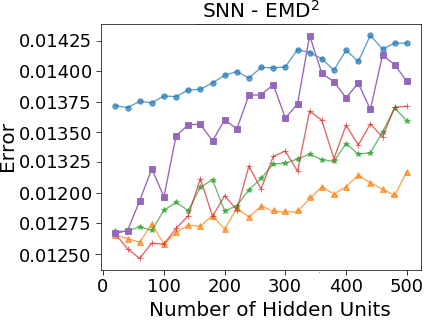
\includegraphics[width=.45\linewidth]{MSE-All-SNN}
			\label{fig:RoomA-MSE-All}}
		\subfloat[Loss of DNN in $\mathcal{A}_1$] {
			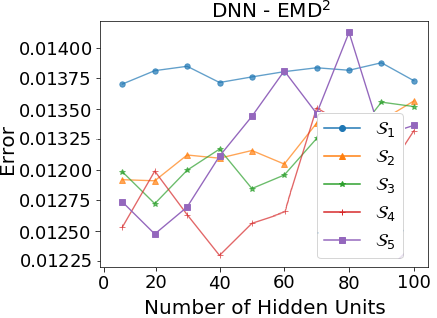
\includegraphics[width=.45\linewidth]{MSE-All-DNN}
			\label{fig:RoomA-DNN-MSE-All}}
		\caption{Feature set and hidden unit size selection based on the generalization error in $\mathcal{A}_1$}
	\end{figure}
	% \begin{figure}[h]
	% 	\centering
	% 	\begin{minipage}[b]{\columnwidth}
	% 		\centering
	% 		\includegraphics[scale=0.35]{"Ortakoy/Mean-of-Means/Pred-Test-4-mini-3"}
	% 		\caption{Predictions of SNN for the Test Fingerprints in the Room A}
	% 		\label{fig:Pred-Test-4}
	% 	\end{minipage}
	% 	\begin{minipage}[b]{\columnwidth}
	% 		\centering
	% 		\includegraphics[scale=0.35]{"Ortakoy/DNN/10_100/Pred-Test-4-mini-3"}
	% 		\caption{Predictions of DNN for the Test Fingerprints in the Room A}
	% 		\label{fig:RoomA-DNN-Pred-Test-4}
	% 	\end{minipage}
	% \end{figure}
	
	%Predictions for $\mathcal{A}_2$ test fingerprints, as we can see in \figurename~\ref{fig:Room B-Pred-Test-3}, \figurename~\ref{fig:Room B-DNN-Pred-Test-3}, fit to the original distribution worse than the predictions for $\mathcal{A}_1$ test fingerprints do. 
	\begin{figure}[h]
		\centering
		\subfloat[Loss of SNN in $\mathcal{A}_2$]{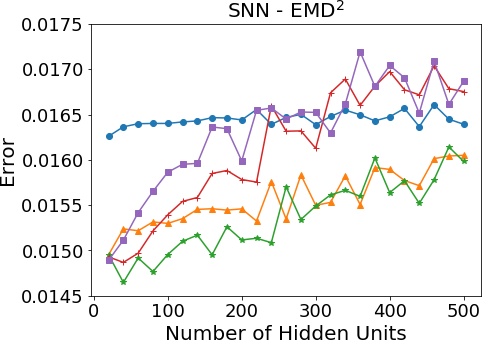
\includegraphics[width=.45\linewidth]{MSE-All-SNN-Lab8}
			\label{fig:RoomB-MSE-All}}
		\subfloat[Loss of DNN in $\mathcal{A}_2$] {
			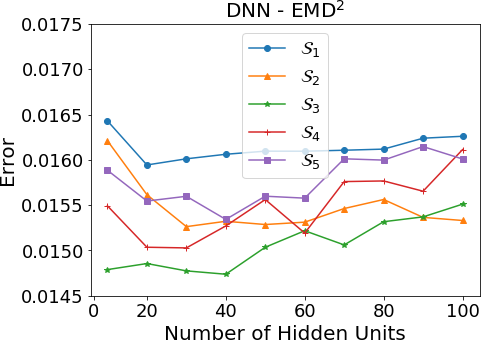
\includegraphics[width=.45\linewidth]{MSE-All-DNN-Lab8}
			\label{fig:RoomB-DNN-MSE-All}}
		\caption{Feature set and hidden unit size selection based on the generalization error in $\mathcal{A}_2$}
	\end{figure}
	
	We expect to predict the RSSI distributions on unknown positions. Examples of distribution predictions are given in \figurename~\ref{fig:predictions}. Calculated with the weights of the best generalized model, the predictions for the test fingerprints do not resemble the original distribution in each and every position. 
	\begin{figure}[h]
		\centering
		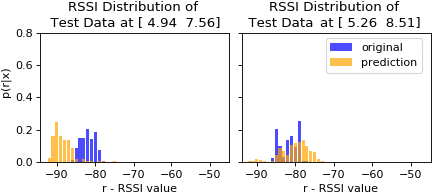
\includegraphics[width=0.8\linewidth]{Pred-Test-3-mini-3}
		
		\caption{Distribution estimation examples}
		\label{fig:predictions}
	\end{figure} 
	
	
	To evaluate sufficiency of radio maps estimated with the neural network for the tracking purpose, we report the trajectory estimation error. We first make estimations of probabilistic RMs over the entire test area by constructing a fine grid of measurement positions chosen at 0.1 meter intervals \cite{Ser2017}. Then we use these constructed maps as the observation distributions in the SMC filter to estimate the trajectory points (for details on the SMC filter see \cite{Ser2017}). To get a more reliable score, 30 radio maps are constructed and used to calculate the tracking accuracy. For both areas, we generate 3 sets of 30 radio maps. One set is generated with all fingerprint data collected, whereas the others are generated with 70\% randomly selected fingerprints, 70\% actively selected fingerprints. We apply particle filtering with 2000 particles and 400 trajectory points in the $\mathcal{A}_1$ and $\mathcal{A}_2$. Filtering is performed once for each RM and each time particles are initialized randomly. This prevents us from getting poor performance because of unfortunate initialization scenarios.
	
	We report the performance of the methods as median tracking error instead of the mean absolute error, because errors form skewed distributions which are clearly non-Gaussian. Constructed with different fingerprint sets with SNN and DNN, tracking accuracy of $\mathcal{A}_1$ and $\mathcal{A}_2$ are given in \figurename~\ref{fig:RoomA-Comparison-Box-NN}. We have three observations. First one is that deep neural networks caused higher median error in both areas. Second one is when the training size is decreased from 100\% to 70\% of data, median error increases. Finally, median errors for the actively selected data is lower than the ones for the randomly selected data on each test area regardless of the neural network type. 
	
	As a final remark from \tablename~\ref{tab:results}, we can reduce the number of training data by 30\% as increasing the tracking accuracy by at most 8.1\% in return. For $\mathcal{A}_1$, the resulting increase are 1.9\% and 2.3\% for SNN and DNN, respectively. For $\mathcal{A}_2$, the resulting increase are 8.1\% and 3.96\%.
	
	\begin{figure}[h]                                                 \subfloat{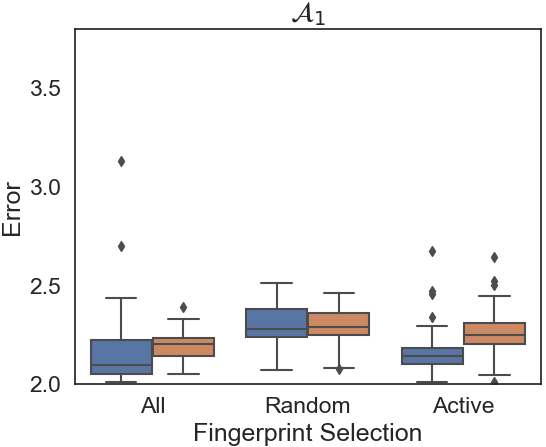
\includegraphics[width=0.5\linewidth]{Ortakoy-Comparison-Box-NN-v6}\label{fig:RoomA-Comparison-Box-NN}}
		\subfloat{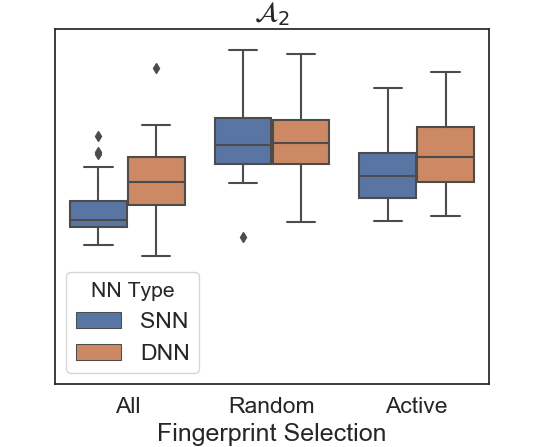
\includegraphics[width=0.5\linewidth]{Lab8-Comparison-Box-NN-v6}\label{fig:RoomB-Comparison-Box-NN}}
		
		\caption{Comparisons of neural network performances in both areas, $\mathcal{A}_1$ and $\mathcal{A}_2$ with various selection strategies. "All" refers to the case of no selection when all collected fingerprints are used.}
	\end{figure}	
	%Comparing the performance of single and two layer NNs in $\mathcal{A}_1$, the DNN gives a lower median accuracy than the SNN with actively selected fingerprints: 2.23 m compared to 2.34 m respectively. Whereas in $\mathcal{A}_2$, using an SNN results in lower localization error than the DNN: 2.94 m compared to 3.11 m in the latter.
	\begin{table}[h]
		\centering
		\resizebox{0.55\columnwidth}{!}{
			\begin{tabular} {| c | c | c | c | c | c | c | c |}
				\hline
				Area & NN type & Fingerprints & 50\% \\ \hline
				\multirow{6}{10pt}{$\mathcal{A}_1$} & \multirow{3}{10pt}{SNN}&All&2.10 \\ \cline{3-4}
				& &Random&2.28 \\ \cline{3-4}
				& &Active&2.14 \\ \cline{2-4} 
				& \multirow{3}{10pt}{DNN}&All&2.20 \\ \cline{3-4}
				&&Random&2.29\\ \cline{3-4}
				&&Active&2.25 \\ \hline
				
				\multirow{6}{10pt}{$\mathcal{A}_2$}&\multirow{3}{10pt}{SNN}&All&2.83 \\ \cline{3-4}
				& &Random&3.21 \\ \cline{3-4}
				& &Active&3.06\\ \cline{2-4}
				&\multirow{3}{10pt}{DNN}&All&3.03\\ \cline{3-4}
				&&Random&3.22\\ \cline{3-4}
				&&Active&3.15\\ \hline
				
		\end{tabular}}
		
		\caption{Accuracy results of NNs in both areas. 50\% corresponds to the second quartile (median) error of positioning error distribution. As the error figures decrease accuracy increases}
		\label{tab:results}
	\end{table}	
	%\begin{table}[h]
	%	\centering
	%	\resizebox{0.75\columnwidth}{!}{
	%		\begin{tabular} {| c | c | c | c | c | c | c | c |}
	%			\hline
	%			Area & NN type & Fingerprints & 50\% & 75\% \\ \hline
	%			\multirow{6}{10pt}{$\mathcal{A}_1$} & \multirow{3}{10pt}{SNN}&All&2.10&2.23 \\ \cline{3-5}
	%			& &Random&2.28&2.38 \\ \cline{3-5}
	%			& &Active&2.14&2.18 \\ \cline{2-5} 
	%			& \multirow{3}{10pt}{DNN}&All&2.20&2.24 \\ \cline{3-5}
	%			&&Random&2.29&2.36 \\ \cline{3-5}
	%			&&Active&2.25&2.31 \\ \hline
				
	%			\multirow{6}{10pt}{$\mathcal{A}_2$}&\multirow{3}{10pt}{SNN}&All&2.83&2.93 \\ \cline{3-5}
	%			& &Random&3.21&3.35 \\ \cline{3-5}
	%			& &Active&3.06&3.17\\ \cline{2-5}
	%			&\multirow{3}{10pt}{DNN}&All&3.03&3.15\\ \cline{3-5}
	%			&&Random&3.22&3.35\\ \cline{3-5}
	%			&&Active&3.15&3.31\\ \hline
				
	%	\end{tabular}}
		
	%	\caption{Accuracy results of NNs in both areas. 50\% corresponds to the second quartile (median) error of positioning error distribution as 75\% corresponds to the third quartile error. As the error figures decrease accuracy increases}
	%	\label{tab:results}
	%\end{table}
	\section{CONCLUSION}
	\label{sec:conclusion}
	%We propose a novel approach consisting of tracking with HMM, radiomap estimation with NN and active selection with GP. 
	We propose a novel approach to reduce the training size required to estimate probabilistic radio maps by picking training positions adaptively. We have two conclusions showing the success of our approach. First one is when we pick the fingerprint positions in an adaptive manner, we estimate fingerprints at remaining locations better than we do with the randomly selected fingerprints in both test areas. Second one is we reduced the training size by $30\%$ with an increase in the median error by 8.1\% at most. Since fingerprinting is a time consuming procedure in indoor localization field, this study would be used to reduce the fingerprinting process of any other methodology in the indoor localization research area.
	
	\vfill\pagebreak
	
	%\section{REFERENCES}
	%\label{sec:refs}
	%%List and number all bibliographical references at the end of the paper. The references can be numbered in alphabetic order or in order of appearance in the document. When referring to them in the text, type the corresponding reference number in square brackets as shown at the end of this sentence \cite{C2}. An additional final page (the fifth page, in most cases) is allowed, but must contain only references to the prior literature.
	
	% References should be produced using the bibtex program from suitable
	% BiBTeX files (here: strings, refs, manuals). The IEEEbib.bst bibliography
	% style file from IEEE produces unsorted bibliography list.
	% -------------------------------------------------------------------------
	\bibliographystyle{styles/IEEEbib}
	\bibliography{references}
	
\end{document}




%\par Constructed with different fingerprint sets with SNN and DNN, tracking accuracy of Room A and Room B are in \figurename~\ref{fig:RoomA-Comparison-Box-NN}. We observed that when the training size is decreased from 100\% to 70\% of data, median error increases. However, when the training fingerprints are selected with uncertainty sampling instead of randomly, we get lower median error. Compared to the results in Room A, median errors are a bit higher in Room B. However, we can again see the decreasing effect of active selection on the median error.
%\begin{figure}[h]
%	\centering
%	\begin{minipage}[b]{\columnwidth}
%		\includegraphics[width=\columnwidth]{"Tracking Errors/Comparison-Box-NN-3"}
%		\caption{Positioning Error on Different Neural Networks with Fingerprint Selection Strategy}
%		\label{fig:RoomA-Comparison-Box-NN}
%	\end{minipage}
%\end{figure}
